\let\negmedspace\undefined
\let\negthickspace\undefined
\documentclass[journal]{IEEEtran}
\usepackage[a5paper, margin=10mm, onecolumn]{geometry}
%\usepackage{lmodern} % Ensure lmodern is loaded for pdflatex

\setlength{\headheight}{1cm} % Set the height of the header box
\setlength{\headsep}{0mm}     % Set the distance between the header box and the top of the text

\usepackage{gvv-book}
\usepackage{gvv}
\usepackage{cite}
\usepackage{amsmath,amssymb,amsfonts,amsthm}
\usepackage{algorithmic}
\usepackage{graphicx}
\usepackage{textcomp}
\usepackage{xcolor}
\usepackage{txfonts}
\usepackage{listings}
\usepackage{enumitem}
\usepackage{mathtools}
\usepackage{gensymb}
\usepackage{comment}
\usepackage[breaklinks=true]{hyperref}
\usepackage{tkz-euclide} 
\usepackage{listings}
\def\inputGnumericTable{}                                 
\usepackage[latin1]{inputenc}                                
\usepackage{color}                                            
\usepackage{array}                                            
\usepackage{longtable}                                       
\usepackage{calc}                                             
\usepackage{multirow}                                         
\usepackage{hhline}                                           
\usepackage{ifthen}                                           
\usepackage{lscape}
\begin{document}

\bibliographystyle{IEEEtran}
\vspace{3cm}

\title{1.11.12}
\author{AI25BTECH11006 - Nikhila}
% \maketitle
% \newpage
% \bigskip
{\let\newpage\relax\maketitle}


\renewcommand{\thefigure}{\theenumi}
\renewcommand{\thetable}{\theenumi}
\setlength{\intextsep}{10pt} % Space between text and floats


\numberwithin{equation}{enumi}
\numberwithin{figure}{enumi}
\renewcommand{\thetable}{\theenumi}


\textbf{Question:} Find the sine of the angle between the vectors  $\vec{a} = 3\hat{i} + \hat{j} + 2\hat{k}$ and\\
\hspace*{1em} $\vec{b} = 2\hat{i} - 2\hat{j} + 4\hat{k}.$

\vspace{2em}

\textbf{Solution:}


The given vectors are $\vec{a} = \myvec{3 \\ 1 \\ 2}, \vec{b} = \myvec{2 \\ -2 \\ 4}.$

We know that 
\begin{align}
|\vec{a}\times\vec{b}| = |\vec{a}| \hspace{0.3em} |\vec{b}|\sin\theta \\
\sin\theta = \frac{|\vec{a}\times \vec{b}|}{|\vec{a}||\vec{b}|}.
\end{align}

\begin{align}
\vec{a} \times \vec{b} = \myvec{3 \\ 1 \\ 2} \times \myvec{2 \\ -2 \\ 4}
 =  8\myvec{1 \\ 1 \\ -1}.
\end{align}

\begin{align}    
|\vec{a}\times\vec{b}| =  \left| 8\myvec{1 \\ 1 \\ -1} \right|  =  8\sqrt{3}.
\end{align}

\begin{align}
|\vec{a}| &= \sqrt{(3)^2 + (1)^2 + (2)^2} = \sqrt{14}, \\
|\vec{b}| &= \sqrt{(2)^2 + (-2)^2 + (4)^2} = \sqrt{24}.
\end{align}

\begin{align}
\sin\theta &= \frac{|\vec{a} \times \vec{b}|}{|\vec{a}||\vec{b}|} \\
&= \frac{8\sqrt{3}}{\sqrt{14}\cdot \sqrt{24}} \\
&= \frac{2}{\sqrt{7}}.
\end{align}


\begin{figure}[h!]
   \centering
   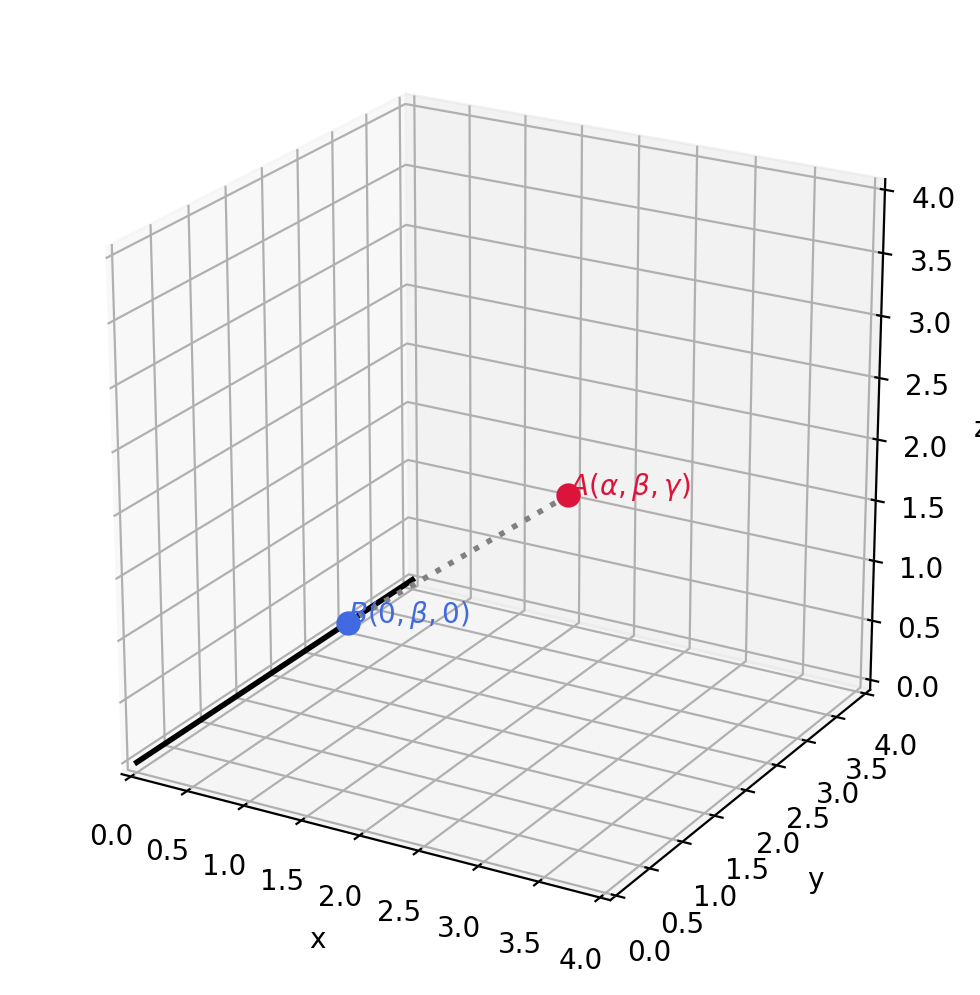
\includegraphics[width=1\linewidth]{fig1.png}
   \caption{}
   \label{stemplot}
\end{figure}


\end{document}

